\subsection{Data Fetching}
\label{subsec:data_fetching}

Data for Validation from MIMIC4:
5508 records each containing 37795 values corresponding to ~605 seconds (fs=64.4725);

Data for Training/Testing from MIMIC3:
22083 (~4*MIMIC4) records each containing 75625 values corresponding to 605 seconds (fs=125);

\subsection{Feature Extraction}
\label{subsec:feature_extraction}

\begin{table}
    \renewcommand{\arraystretch}{1.5}
    \setlength{\tabcolsep}{12pt}
    \begin{center}
        \begin{tabular}{ |c|c|c| }
            \hline
            & MIMIC-III  & MIMIC-IV  \\
            \hline
            Records       & 22,083     & 5,508     \\
            \hline
            Total Values  & 13,659,375 & 1,309,265 \\
            \hline
            Median Values & 1,918,623  & 183,140   \\
            \hline
        \end{tabular}
    \end{center}
    \captionsetup{format=plain, justification=centering}
    \caption{Fetched and Extracted Data from MIMIC-III and MIMIC-IV DBs}
    \label{tab:records}
\end{table}

FE from MIMIC4 for Validation:
- For target reference Systolic, Diastolic and MAP values were extracted from the waveform data.
- For Machine Learning, 34 features were extracted from the PPG waveform
A total of \textbf{1,309,265} values were extracted, resulting in a 34 x 1,309,265 matrix.
Total of \textbf{183,140} median values were extracted.

FE from MIMIC3 for Training/Testing:

- For target reference ABP Systolic, Diastolic and MAP values were extracted from the waveform data.
- For Machine Learning, 34 features were extracted from the PPG waveform
A total of \textbf{13,659,375} values were extracted, resulting in a 34 x 13659375 matrix.
Total of \textbf{1,918,623} median values were extracted.

The summarized results are displayed in Table~\ref{tab:records}.
Data Flow is visualized in Figure~\ref{fig:data_flow}.

\begin{figure}[h]
    \centering
    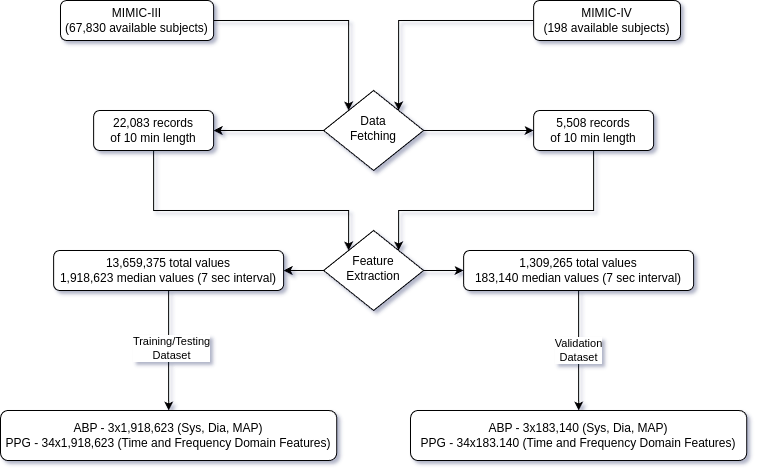
\includegraphics[width=0.9\textwidth]{images/results/flow_diagram}
    \caption{Flow Diagram presenting the Data Fetching and Processing}
    \label{fig:data_flow}
\end{figure}

\subsection{Machine Learning}
\label{subsec:machine_learning}

As mentioned in previous chapters, an ideal ratio of 60/20/20 train/test/validate was aimed for.
However in the end having 1,918,623 values from MIMIC-III and 183,140 values from MIMIC-IV, a different approach was taken.
the MIMIC-III data was used for training/testing, and it was split into 80/20 train/test, resulting in 1,534,898 training and 383,725 testing datapoints.
Therefore final train/test/validate proportions were 1,534,898 / 383,725 / 183,140 - 73 / 18 / 9.
% possibly discussion
All this means is that the signal processing algorithms worked better and extracted more values from the MIMIC-III DB.
It is also possible a hint at the fact, that the quality of the signal was better in MIMIC-III.
This is also logical however, since there was no limit on the fetching of records from a single study or subject from MIMIC-IV,
so huge number of segments might have been discarded, if they didn't showcase a comprehensible signal.

\begin{center}
    \begin{tabular}{ |c|c|c|c| }
        \hline
        & Training Loss (MSE) & Testing Loss (MSE) & Testing MAE \\
        \hline
        LR                     & 218.443             & -                  & 11.097      \\
        \hline
        MLP                    & 208.343             & -                  & 10.866      \\
        \hline
        LSTM                   & 93.81               & 97.358             & 6.953       \\
        \hline
        LSTM (weight adjusted) & 97.615              & 100.498            & 7.085       \\
        \hline
        Bi-LSTM                & -                   & -                  & -           \\
        \hline
        GRU                    & 88.34               & 92.142             & 6.759       \\
        \hline
        GRU (weight adjusted)  & 88.167              & 90.955             & 6.727       \\
        \hline
        Bi-GRU                 & -                   & -                  & -           \\
        \hline
        SVR                    & -                   & -                  & -           \\
        \hline
        RF                     & -                   & -                  & -           \\
        \hline
    \end{tabular}
\end{center}

\begin{center}
    \begin{tabular}{ |c|c|c|c| }
        \hline
        & Testing RMSE & Validation RMSE & Validation MAE \\
        \hline
        LR                     & 14.777       &                 &                \\
        \hline
        MLP                    & 14.446       &                 &                \\
        \hline
        LSTM                   & 9.866        & -               & 14.597         \\
        \hline
        LSTM (weight adjusted) & 10.024       & -               & 14.646         \\
        \hline
        Bi-LSTM                & -            & -               & -              \\
        \hline
        GRU                    & 9.598        & -               & 14.951         \\
        \hline
        GRU (weight adjusted)  & 9.536        & -               & 15.205         \\
        \hline
        Bi-GRU                 & -            & -               & -              \\
        \hline
        SVR                    & -            & -               & -              \\
        \hline
        RF                     & -            & -               & -              \\
        \hline
    \end{tabular}
\end{center}

LSTM \& GRU training and testing loss charts (32 \& 33) % (\ref{fig:train_mse} \& \ref{fig:test_mse}).

It was found, that every feature contributes positively, therefore feature reduction was not applied.
Feature Importance chart in Figure~34 (at the end of the document) % \ref{fig:feat_importance} (at end of document).

%\begin{figure}
%    \centering
%    \begin{subfigure}{0.5\textwidth}
%        \centering
%        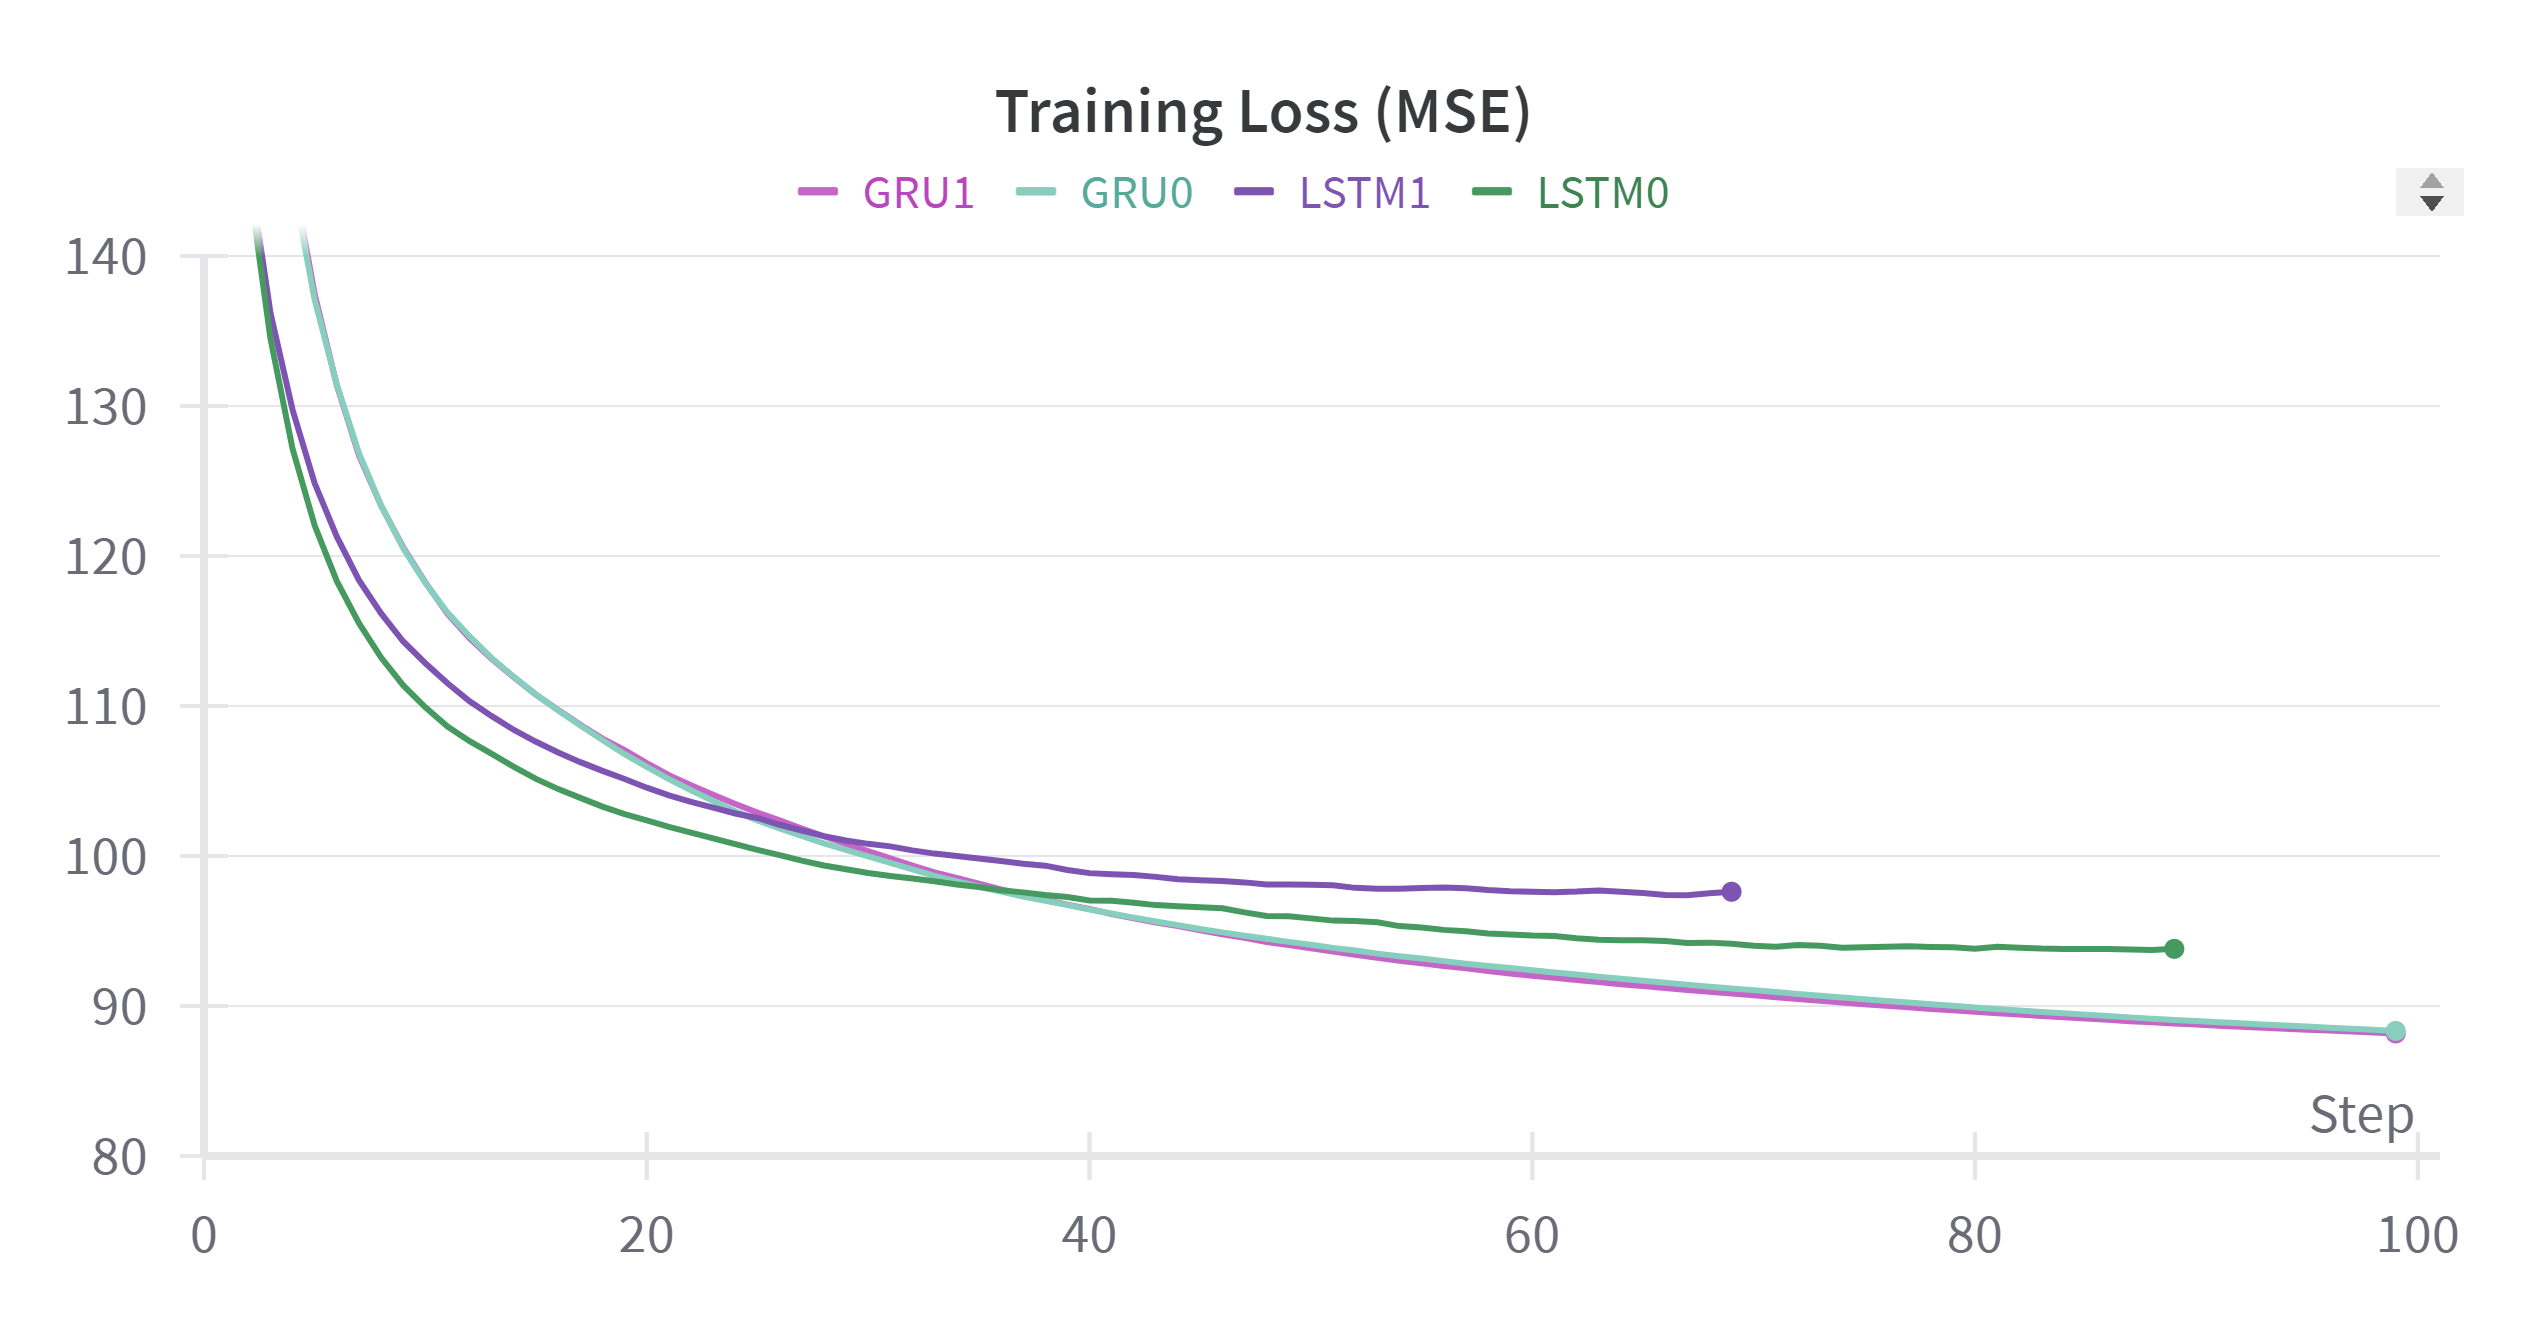
\includegraphics[width=0.4\linewidth]{images/results/LSTM_GRU_Train_mse}
%        \caption{LSTM \& GRU Train MSE}
%        \label{fig:train_mse}
%    \end{subfigure}
%    \begin{subfigure}{0.5\textwidth}
%        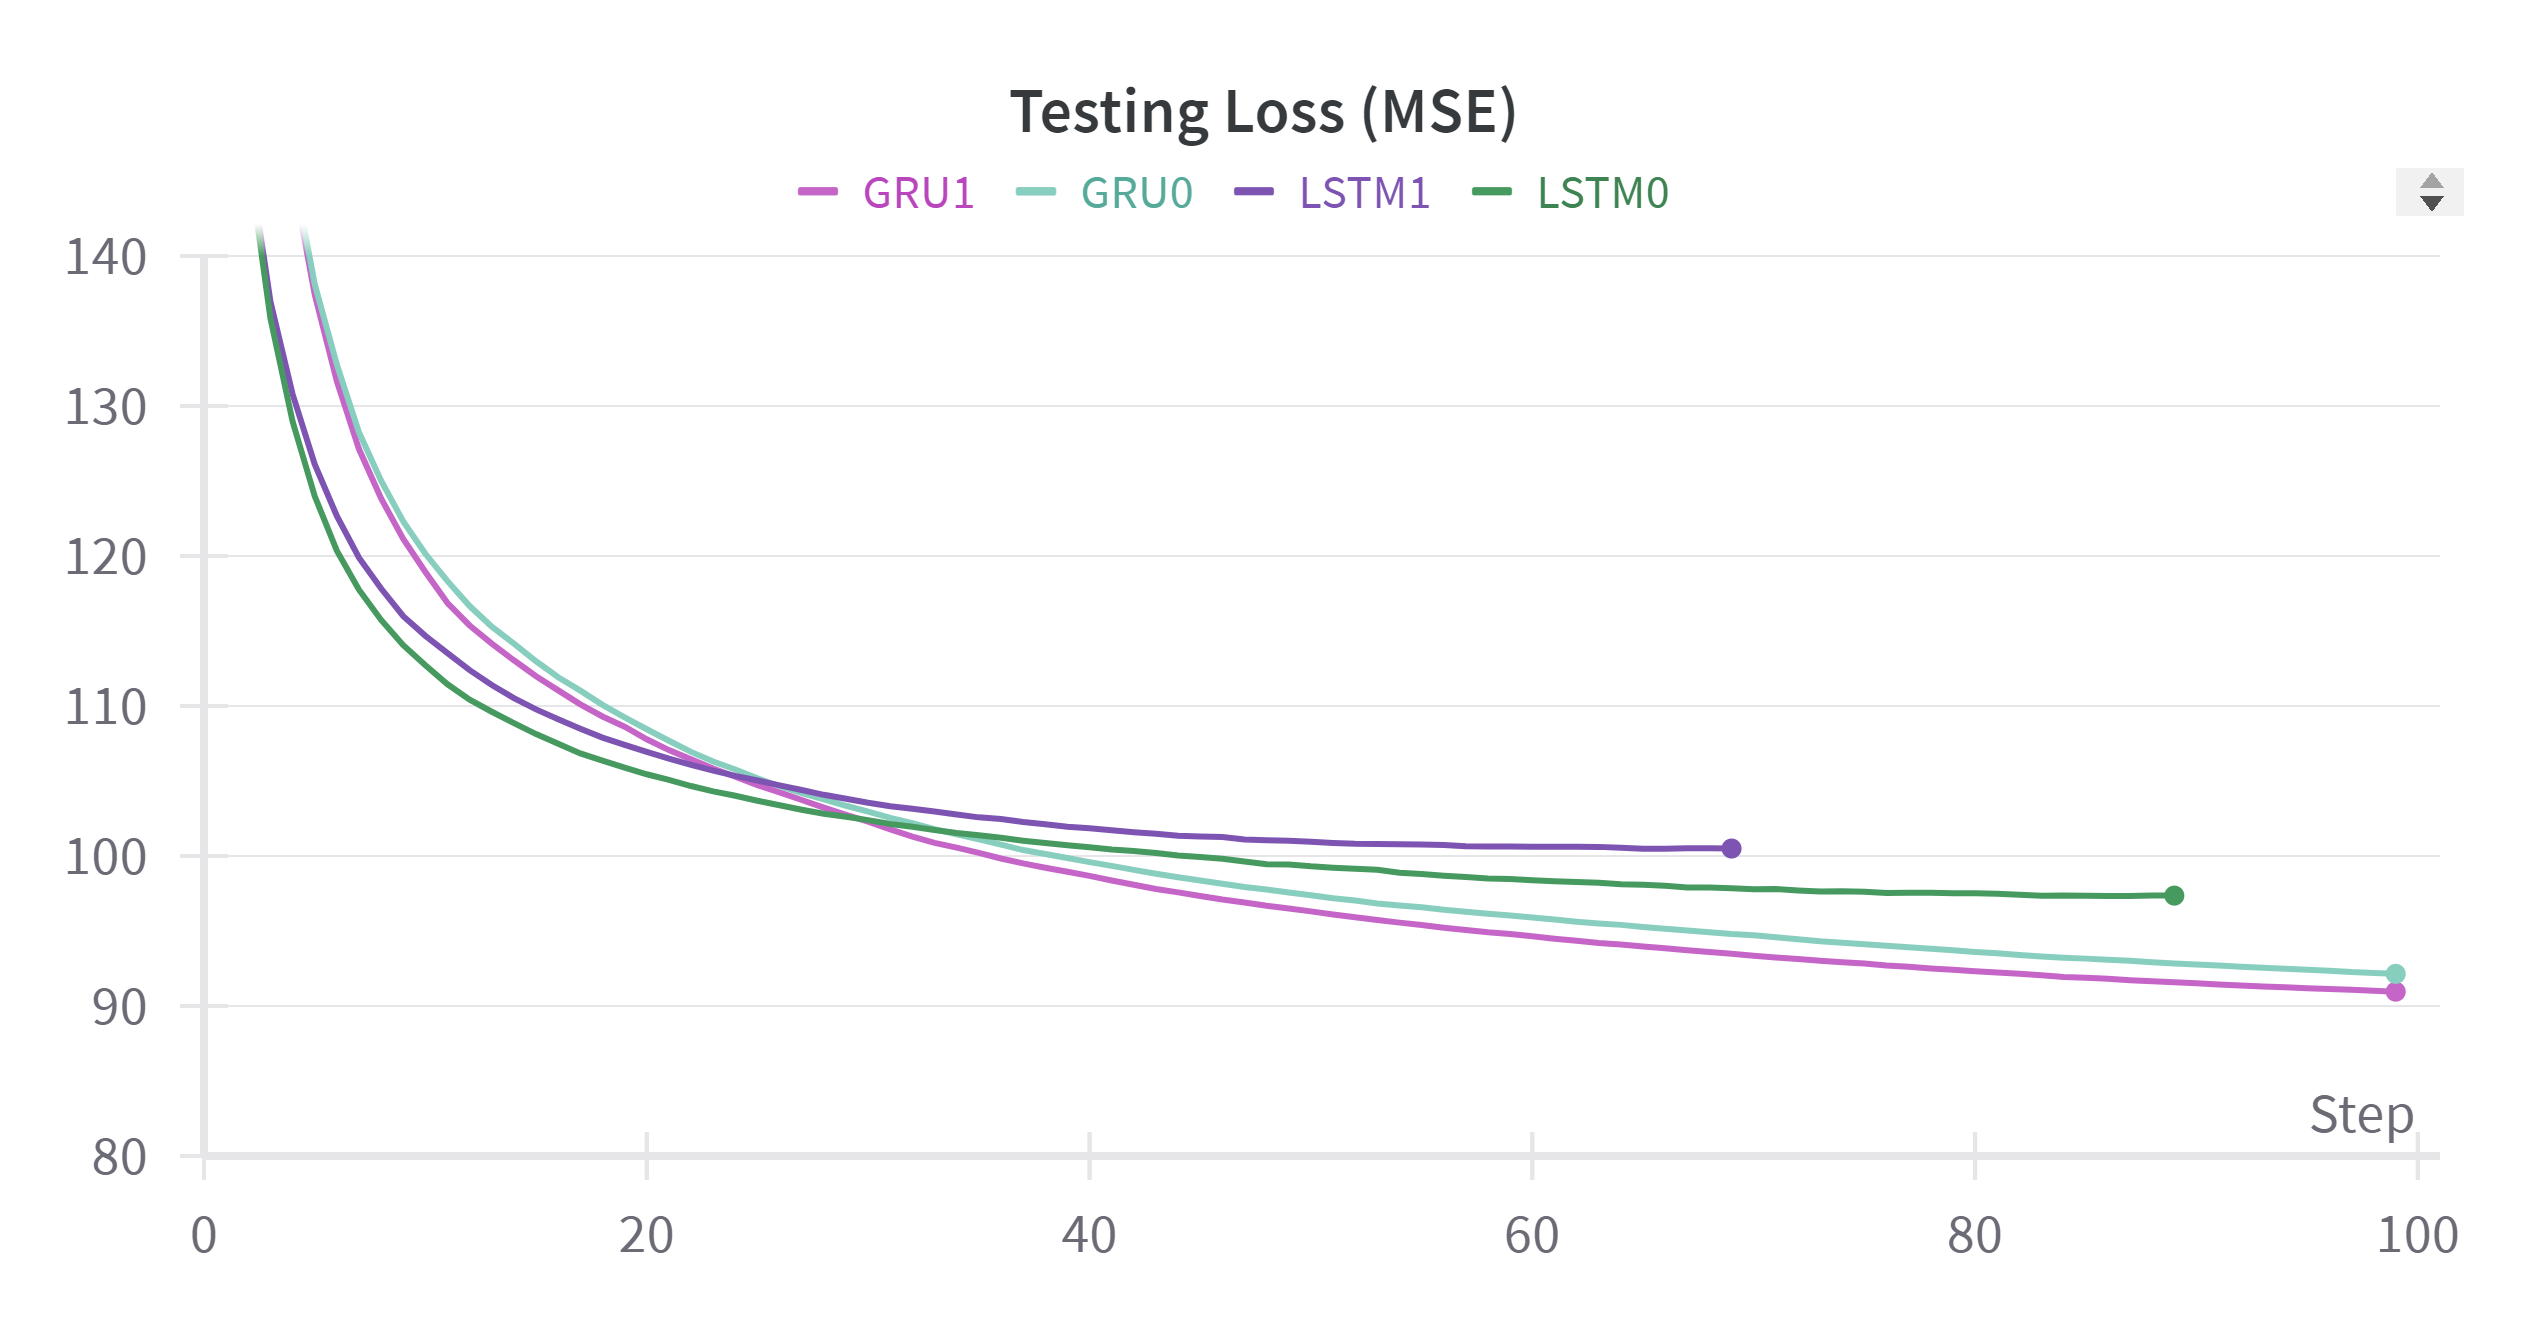
\includegraphics[width=0.4\linewidth]{images/results/LSTM_GRU_Test_mse}
%        \caption{LSTM \& GRU Test MSE}
%        \label{fig:test_mse}
%    \end{subfigure}
%\end{figure}

\begin{figure}[h]
    \centering
    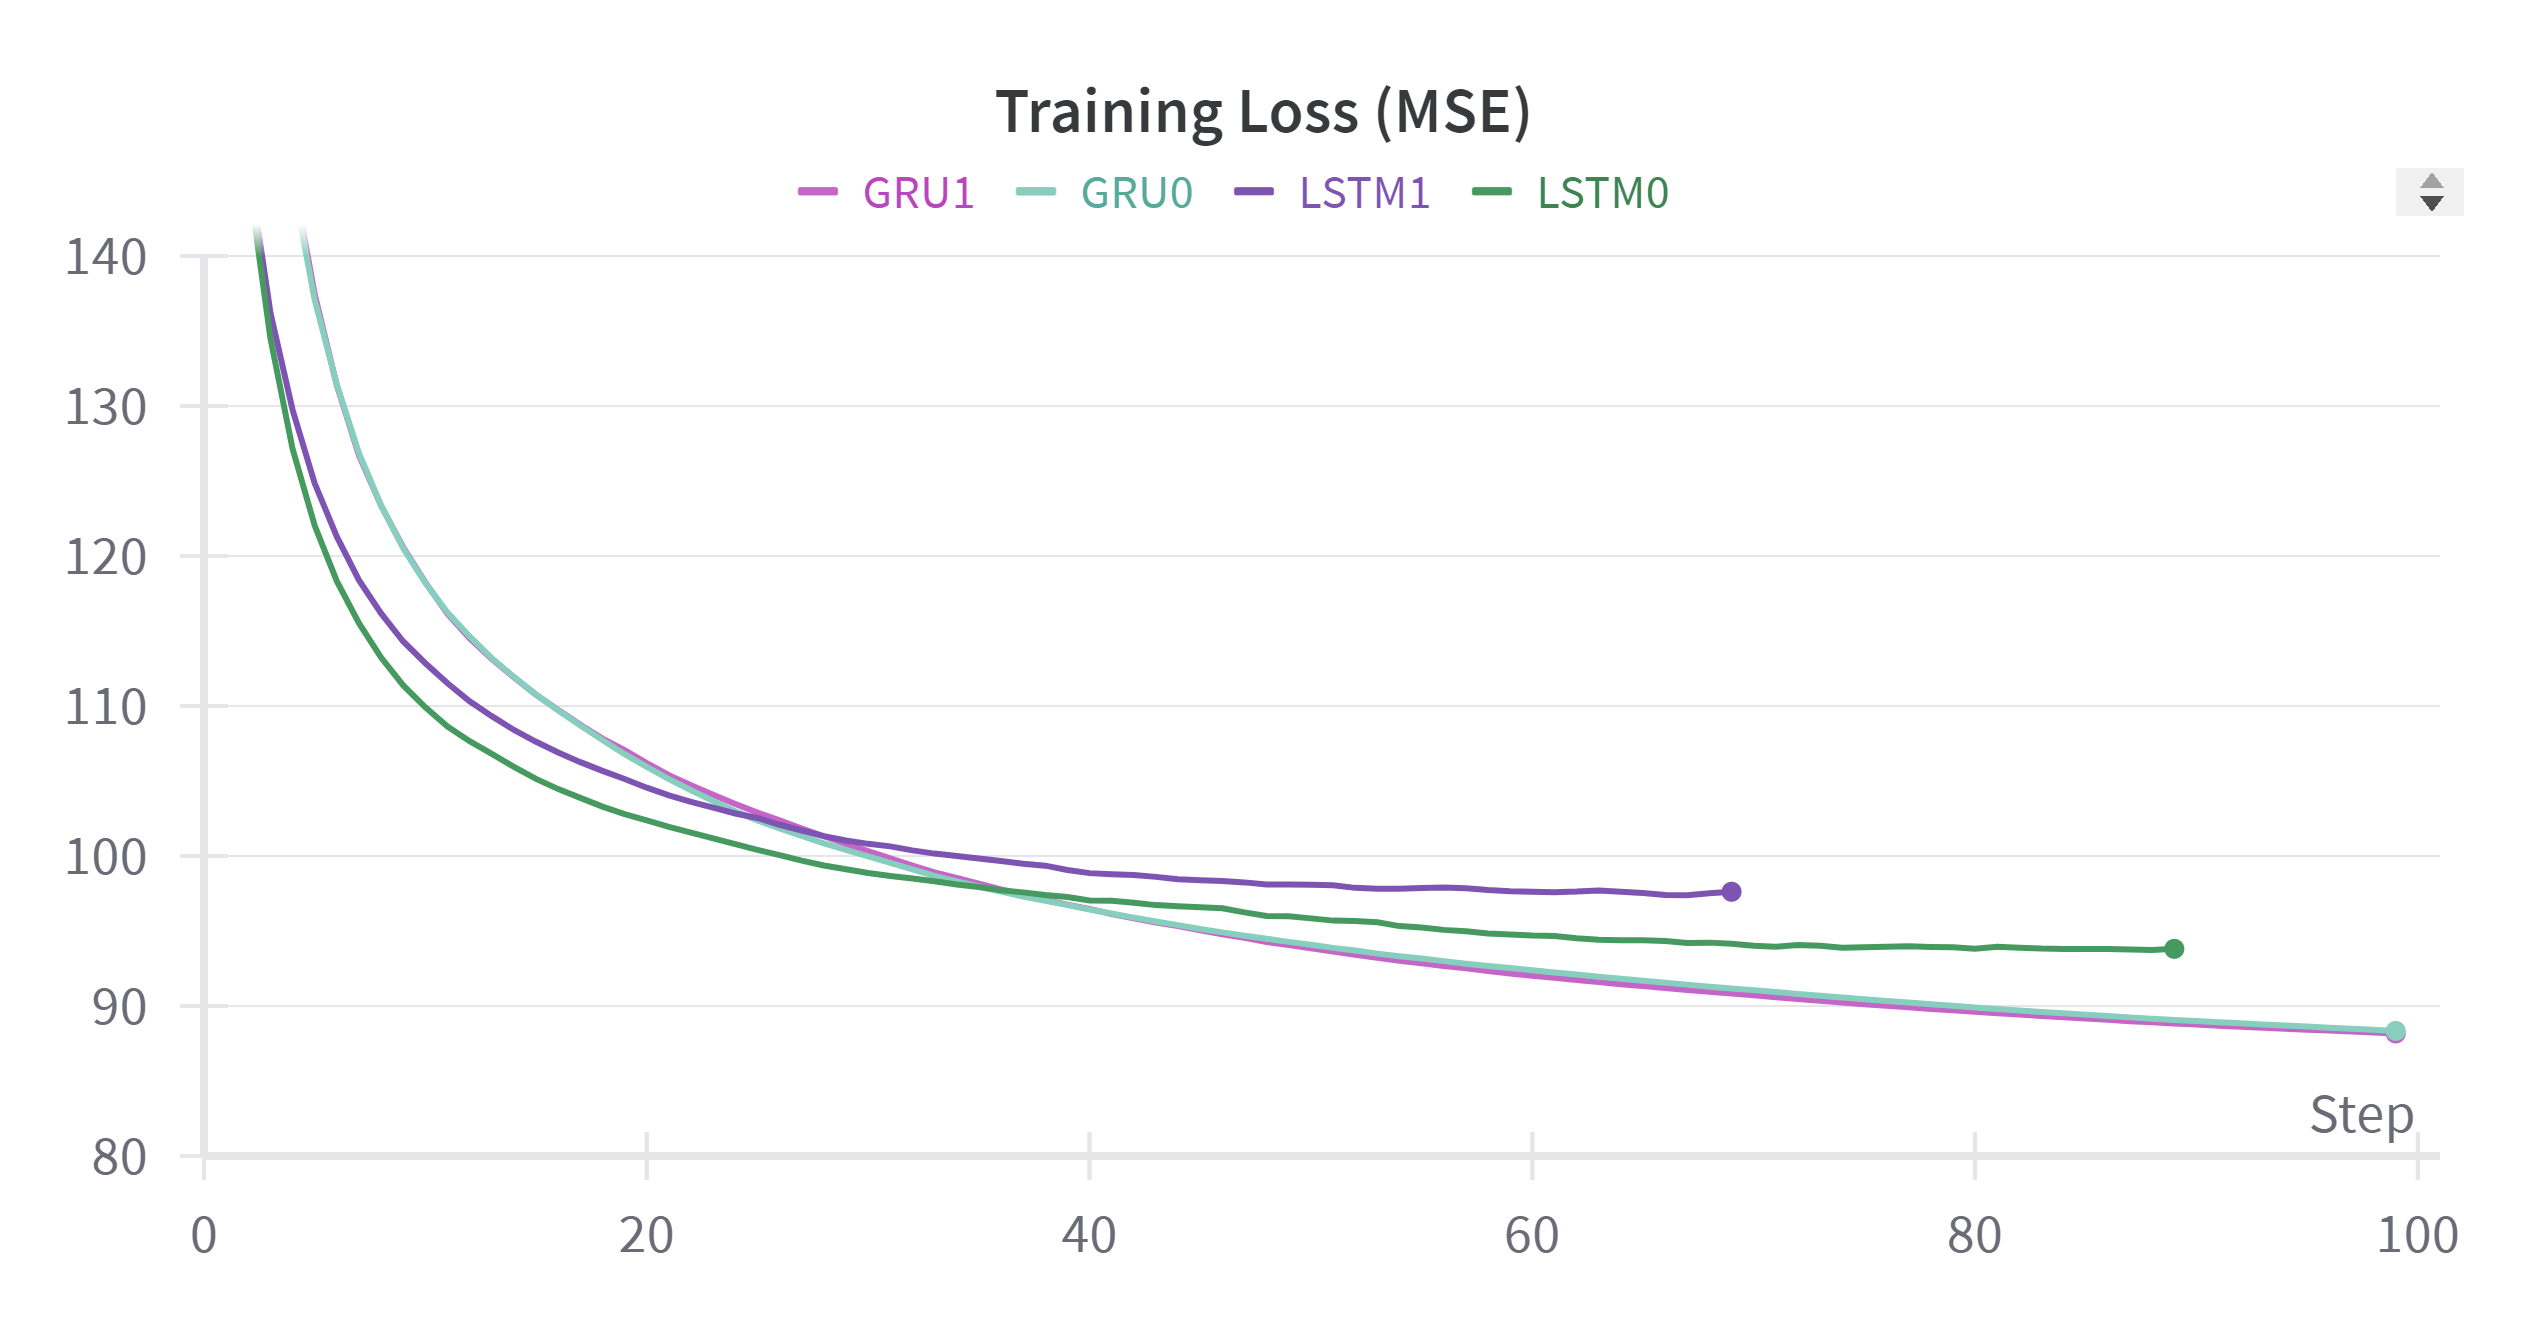
\includegraphics[width=0.4\linewidth]{images/results/LSTM_GRU_Train_mse}
    \caption{LSTM \& GRU Train MSE}
    \label{fig:train_mse}
\end{figure}

\begin{figure}[h]
    \centering
    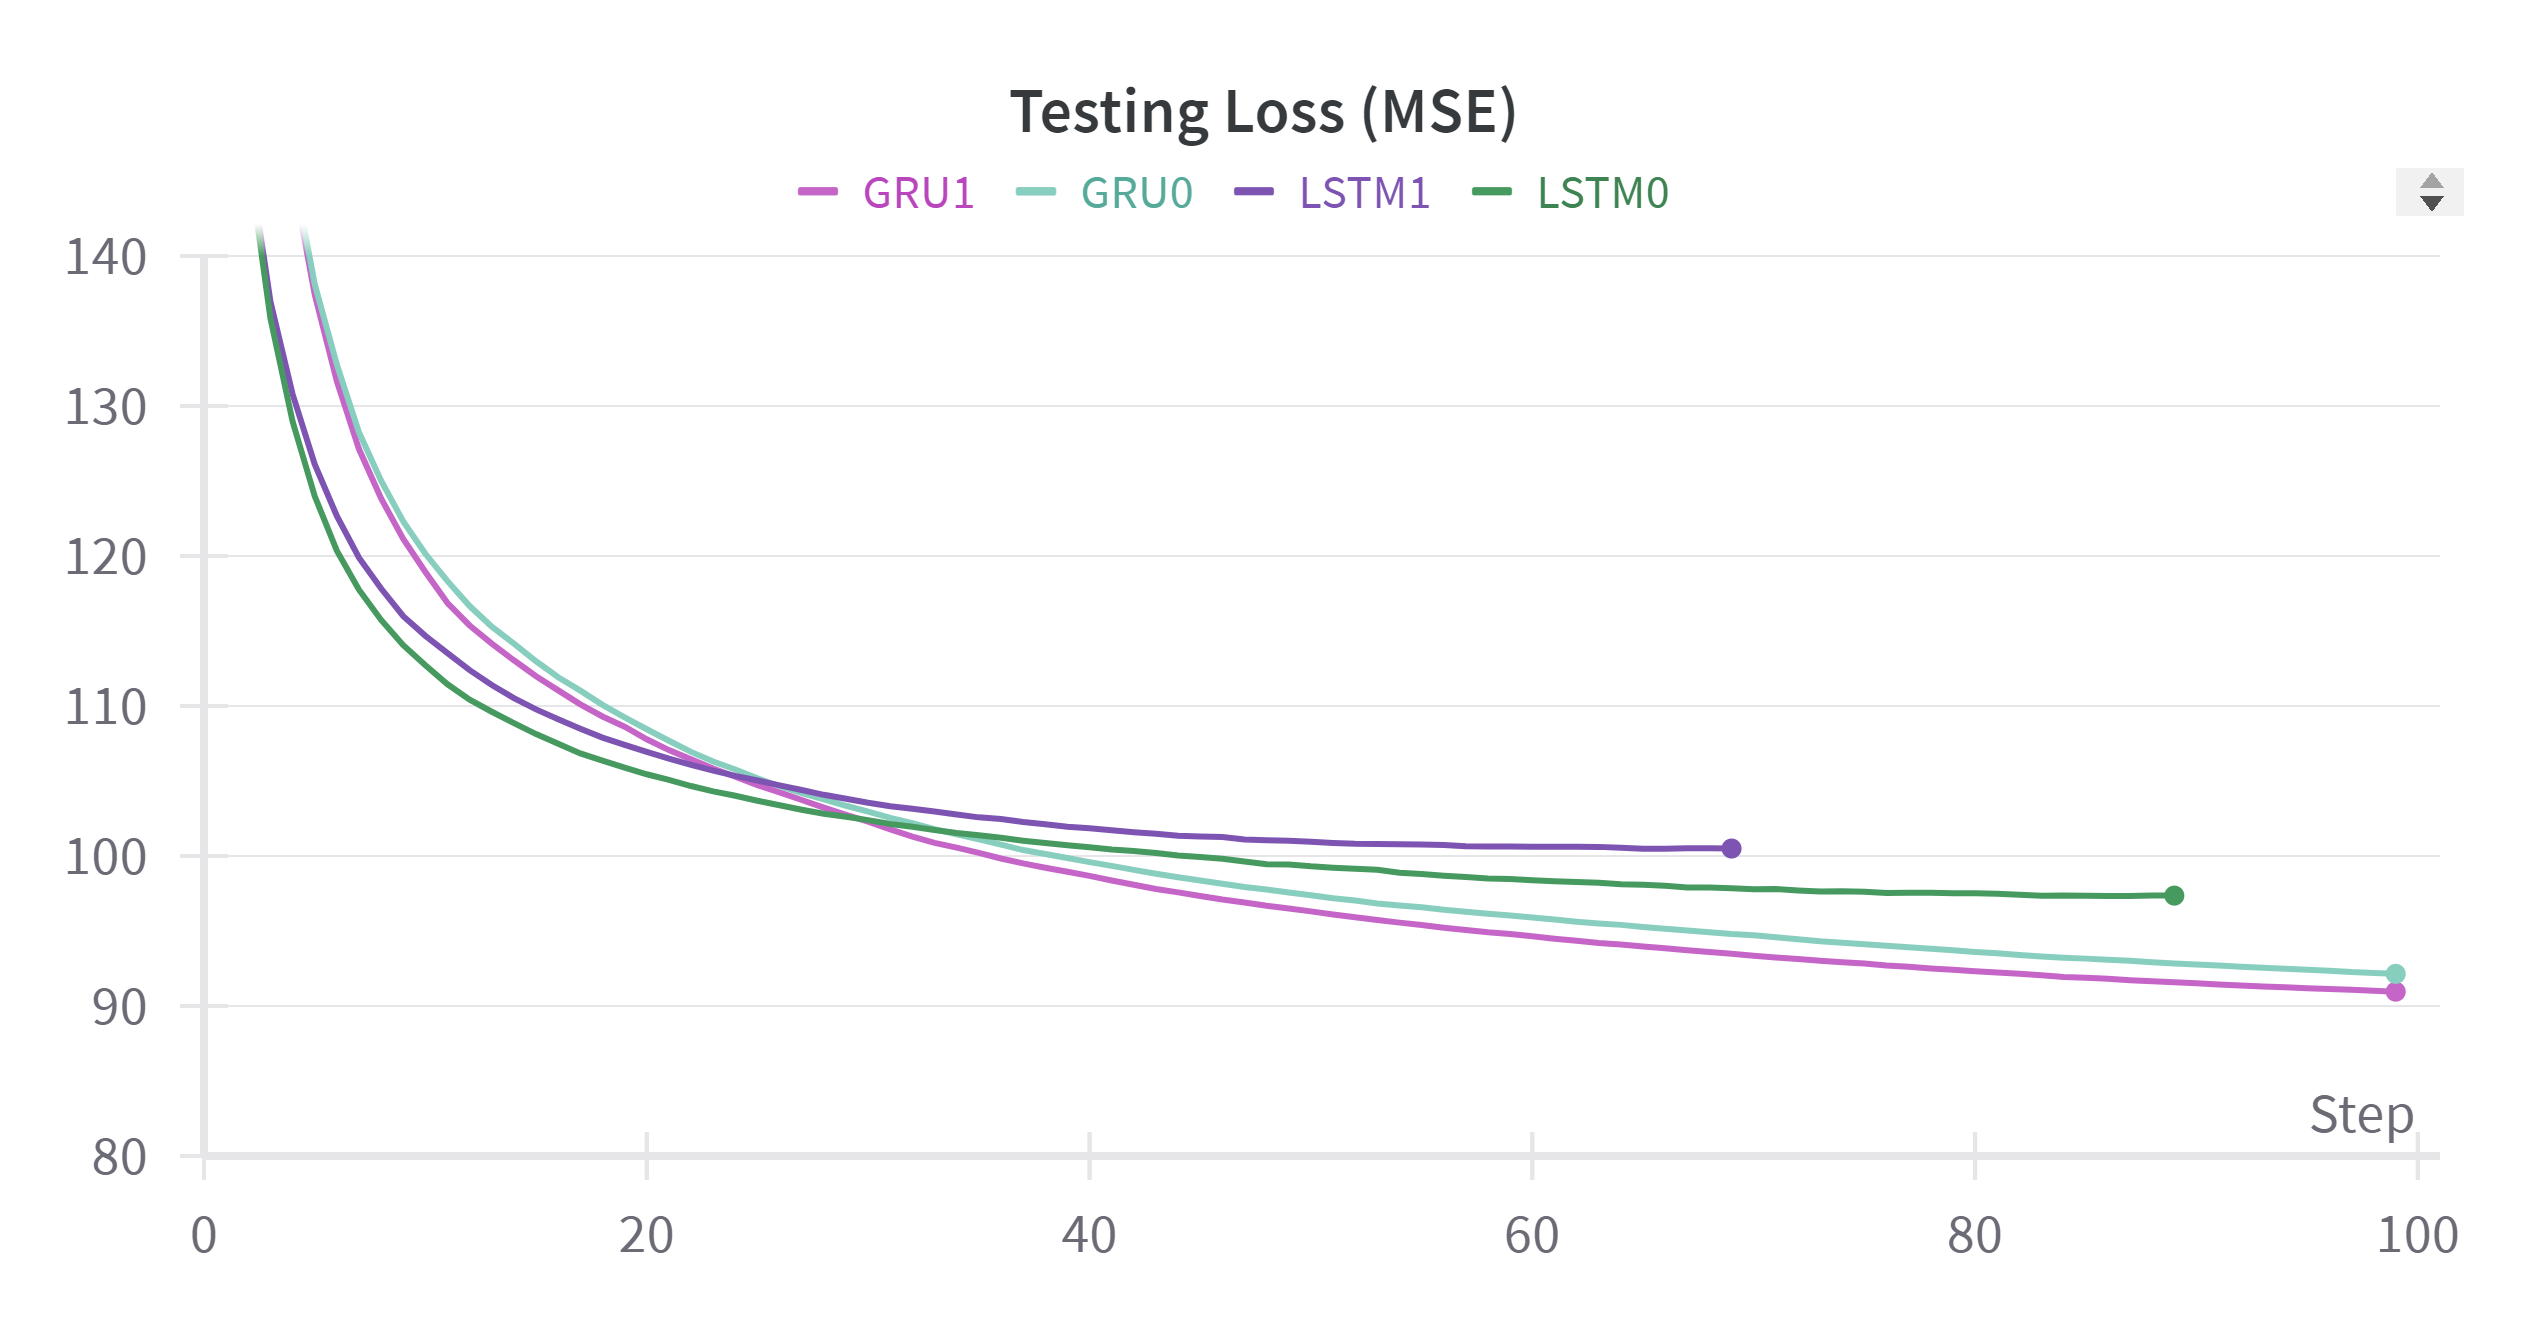
\includegraphics[width=0.4\linewidth]{images/results/LSTM_GRU_Test_mse}
    \caption{LSTM \& GRU Test MSE}
    \label{fig:test_mse}
\end{figure}

\begin{figure}[h]
    \centering
    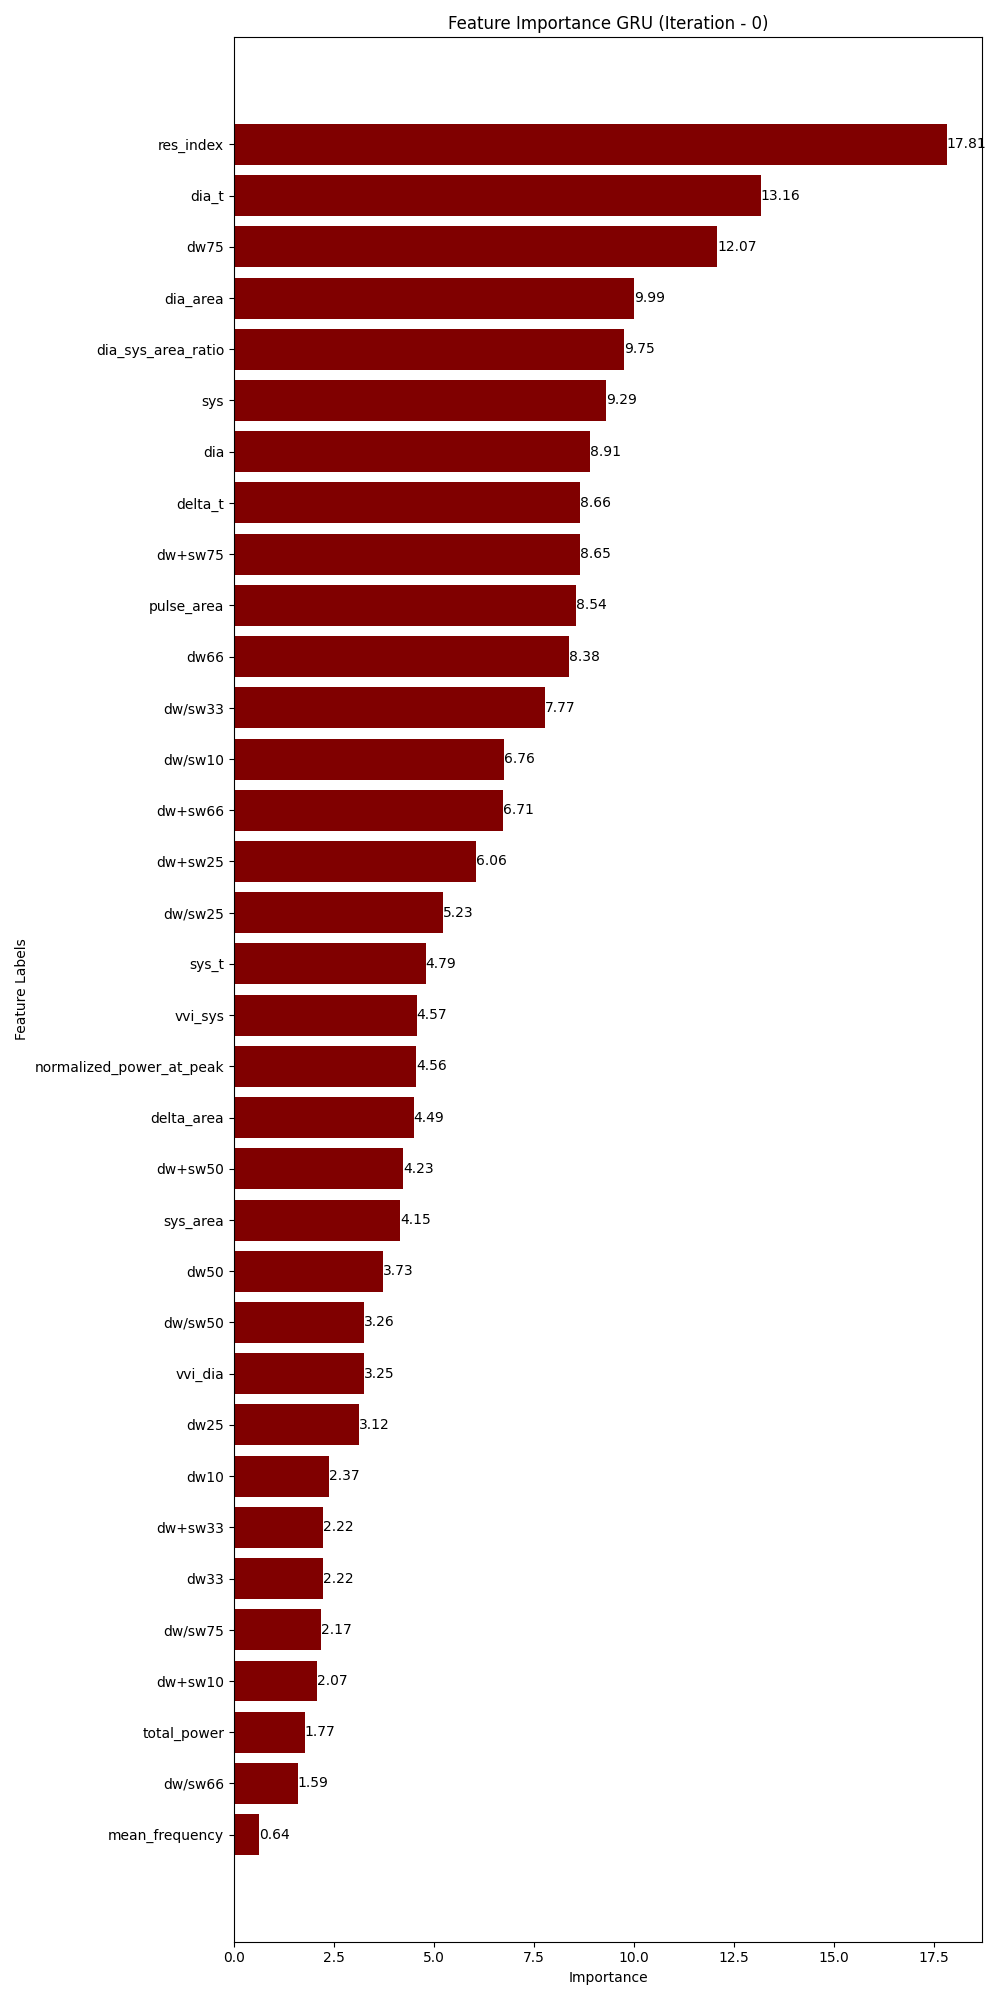
\includegraphics[width=0.5\textwidth]{images/results/feature_importance_plot_GRU_0}
    \caption{Feature Importance Chart}
    \label{fig:feat_importance}
\end{figure}
